%!TEX TX-program = xelatex
\documentclass[8pt]{article}

\usepackage[UTF8]{ctex}
\usepackage{graphicx}
\usepackage{enumerate}
\usepackage{geometry}
\usepackage{amsmath}
\usepackage{amssymb}
\usepackage{amsfonts}
\usepackage{tikz}
\usetikzlibrary{positioning}
\usepackage{xcolor}

\title{\S 2 集合'}
\author{高一(6)班\ 邵亦成\ 26号}
\date{2021年09月25日}

\geometry{a4paper, scale=0.85}

\begin{document}

	\maketitle

	\begin{enumerate}
		\item

			设$a_1,a_2,\cdots,a_{20}\in \{1,2,3,4,5\}, b_1,b_2,\cdots,b_{20}\in\{1,2,3,\cdots,10\}$,

			集合$X=\left\{(i,j)|i\leq i < j \leq 20, \left(a_i-a_j\right)\left(b_i-b_j\right)<0\right\}$,求$|X|_{\max}$.

			~\\
			最优情况必为$a_n$递增,$b_n$递减.

			易证$\left\{(i,j)|a_i=a_j\right\}\cap X = \emptyset$,

			即求$\left|\left\{(i,j)|a_i=a_j\right\}\right|_{\min}.$

			不妨设$a_1\leq a_2 \leq \cdots \leq a_{20}$,

			设其中值为$i$的数有$X_i$个$(i=1,2,3,4,5)$,则有$X_1+X_2+X_3+X_4+X_5=20$.

			结合Cauchy不等式,有

			$$
				\begin{array}{rl}
					&\left|\left\{(i,j)|a_i=a_j\right\}\right| \\
					=&C_{X_1}^2+C_{X_2}^2+\cdots+C_{X_5}^2\\
					=&\displaystyle{\frac{1}{2}\left[\frac{\left(X_1+X_2+X_3+X_4+X_5\right)^2}{5}-\left(X_1+X_2+X_3+X_4+X_5\right)\right]}\\
					=&\frac{1}{2}\times20\times3\\
					=&30.\\
				\end{array}
			$$

			故$|X|\leq C_{20}^2 - 30 = 160$,

			在

			$$
			\begin{aligned}
			&a_1=a_2=a_3=a_4=1, &a_5=a_6=a_7=a_8=2, &\cdots, &a_{17}=a_{18}=a_{19}=a_{20}=5\\
			&b_1=b_2=b_3=b_4=5, &b_5=b_6=b_7=b_8=4, &\cdots, &b_{17}=b_{18}=b_{19}=b_{20}=1\\
			\end{aligned}
			$$

			时有$|X|_{\max}=160$.

		~\\

		\item

			集合$A,B$有:

			\begin{enumerate}[ (1) ]
				\item $A\cup B=\{3,4,\cdots,n\}$

				\item $A\cap B=\emptyset$

				\item $\forall x,y \in A: x,y \notin A$

				\item $\forall x,y \in B: x,y \notin B.$

			\end{enumerate}

			求$n_{\max}$.

			~\\
			不妨设$3\in A \Rightarrow 9 \in B \Rightarrow 81 \in A \Rightarrow 243 \in B,$但$3\in A, 81\in A \Rightarrow 27\in B \Rightarrow 243\in A$,

			所以有$n\leq242$.

			$$
			A=\{3,4,5,6,7,8,81,82,\cdots,242\}, B=\{9,10,\cdots,80\}
			$$

			时有$n_{\max}=242.$

		~\\

		\item

			$A$和$B$是平面上的两个点,过$A,B$的直线为$l$,由$l$分成的一个半平面内,有$2021$个不同的点$P_1,P_2,P_3,\cdots,P_{2021}$.则由$A,B$到$P_i(i=1,2,\cdots,2021)$的距离所构成的集合中,至少有多少个不同的元素.

			~\\
			设集合中有$n$个元素$r_1,r_2,\cdots,r_n$.以$A,B$为圆心,$r_1,r_2,\cdots,r_n$为半径作半圆.

			$$
			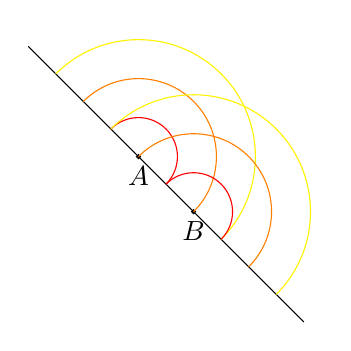
\begin{tikzpicture} [scale=0.35]
				\draw  [black](-5,5)--(5,-5);
				\filldraw [black] (-1,  1) circle (2pt) node[anchor=north] {$A$};
				\filldraw [black] (1 , -1) circle (2pt) node[anchor=north] {$B$};
				\draw [red] (0, 0) arc (-45:135:{sqrt(2)});
				\draw [orange] (1, -1) arc (-45:135:{2*sqrt(2)});
				\draw [yellow] (2, -2) arc (-45:135:{3*sqrt(2)});
				\draw [red] (2, -2) arc (-45:135:{sqrt(2)});
				\draw [orange] (3, -3) arc (-45:135:{2*sqrt(2)});
				\draw [yellow] (4, -4) arc (-45:135:{3*sqrt(2)});
			\end{tikzpicture}
			$$

			$\therefore P_i(i=1,2,\cdots,2021)$在某个半圆上,而半圆至多有$n^2$个交点.

			$\therefore n^2 \geq 2021, n \geq 45.$

		~\\

		\item

			设$P_0, P_1, \cdots, P_n$为平面上的$n+1$个点,它们之间两两间距离的最小值为$d(d>0)$. 

			求证:

			$$\prod_{i=1}^{n}\left|P_0P_i\right|>\left(\frac{d}{3}\right)^n\cdot\sqrt{(n+1)!}\ .$$

			~\\
			从$P_i(i=0,1,2,\cdots,n)$为圆心,$\frac{d}{2}$为半径作$\odot P_i$.

			$\therefore \odot P_i$一定两两外切或外离且至少一组圆外切.

			只需证$\left|P_0P_k\right|>\frac{d}{3}\sqrt{k+1}\ .$

			不妨令$\left|P_0P_1\right|\leq\left|P_0P_2\right|\leq\cdots\leq\left|P_0P_k\right|,$

			若$n\geq8$,以$P_0$为圆心,$\left|P_0P_n\right|+\frac{d}{2}$为半径作圆,则有$\odot P_i$均在大圆内.

			[\ 设$Q$为$\odot P_i$上任意一点,则有:$\left|P_0Q\right|\leq\left|P_0P_i\right|+\left|P_iQ\right|\leq\left|P_0P_n\right|+\frac{d}{2}$.\ ]

			比较面积:

			$$
			\begin{array}{rcl}
				\pi \left[\left|P_0P_n\right|+\frac{d}{2}\right]^2&>&\pi\left(\frac{d}{2}\right)^2\cdot(n+1)\\
				\left|P_0P_n\right|&>&\frac{d}{2}\cdots\left(\sqrt{n+1}-1\right)\\
				&\geq&\frac{d}{3}\sqrt{n+1}\\
				&\Updownarrow&\\
				3\left(\sqrt{n+1}-1\right)&\geq&2\sqrt{n+1}\\
				&\Updownarrow&\\
				\sqrt{n+1}&\geq&3\\
				&\Updownarrow&\\
				n&\geq&8.\\
			\end{array}
			$$

			若$n\leq 7$, $\frac{d}{3}\sqrt{n+1}<d.$

			得证.

		~\\

		\item

			有限集$A\subseteq \mathbb{N}^{*}$. 求证:$\exists$有限集$B: A\subseteq B \subseteq \mathbb{N}^{*}$有

			$$\prod_{x\in B}x=\sum_{x\in B}x^2.$$

			~\\
			不妨令初始状态为$B=A$.

			若$\displaystyle{\prod_{x\in B}x=\sum_{x\in B}x^2}$,则问题解决.

			若$\displaystyle{\prod_{x\in B}x>\sum_{x\in B}x^2}$,则尝试去缩小$\displaystyle{\prod_{x\in B}x-\sum_{x\in B}x^2}$.

			记$\displaystyle{\prod_{x\in B}x=P, \sum_{x\in B}x^2=S, C=P-S, }$

			目标即为在$B$中添加一个元素$y$,使得$C\rightarrow C-1$.

			则有:

			$$
			\begin{array}{rcl}
				P\cdot y - (S + y^2) &=& P - S - 1\\
				-y^2 + P\cdot y - p + 1 &=& 0\\
				P(y-1)&=&(y-1)(y+1).\\
			\end{array}
			$$

			显然,不可能一直添加$1$.

			如果$P-1\in B$,则$B=\{1,2\}$,$P=2, S=3$,与前提假设不符.

			所以有$P-1\notin B$,添加$P-1$即可.

			若$\displaystyle{\prod_{x\in B}x<\sum_{x\in B}x^2}$,

			令$A=\left\{x_1,x_2,\cdots,x_n\right\}\left(x_1<x_2<\cdots<x_n\right)$,

			当$x_n\geq 6时$,令$B=\left\{1,2,\cdots,x_n\right\},则有:$

			$$
				\begin{array}{rl}
					&\displaystyle{\prod_{x\in B}x-\sum_{x\in B}x^2}\\
					=&\displaystyle{\left(x_n\right)!-\frac{x_n\left(x_n+1\right)\left(2x_n+1\right)}{6}}\\
					=&\frac{x_n}{6}\left[6\left(x_n-1\right)!-\left(x_n+1\right)\left(2x_n+1\right)\right]\\
					\geq&\frac{x_n}{6}\left[6\left(x_n-1\right)\left(x_n-2\right)-\left(x_n+1\right)\left(2x_n+1\right)\right]\\
					=&\frac{x_n}{6}\left(4x_n^2-21x_n+11\right)\\
					>&0\\
				\end{array}
			$$

			于是按照$\displaystyle{\prod_{x\in B}x>\sum_{x\in B}x^2}$操作即可.

			当$x_n\leq 5$时,令$B=\left\{1,2,3,4,5,6\right\}$即可.

			$\therefore \forall$有限集$A\subseteq \mathbb{N}^{*} \ \exists$有限集$B: A\subseteq B \subseteq \mathbb{N}^{*}$有

			$$\prod_{x\in B}x=\sum_{x\in B}x^2.$$

		~\\

		\item

			设有$n$个人,任意两人在其他$n-2$人中都至少有2016位共同的朋友,朋友关系是相互的. 求所有的$n$,使得在满足以上所有条件的任何情况下都存在$5$人彼此是朋友.

			~\\
			考虑原命题结论的反面:不存在$5$个人彼此是朋友的$n_{\min}$.

			设$a_1, a_2$是朋友,他们至少有$2016$名共同的朋友$b_1, b_2, \cdots, b_{2016}$,

			若$b_1, b_2, \cdots, b_{2016}$中有一对朋友,不妨设为$b_1, b_2$,

			$b_1, b_2$的共同朋友中,除了$a_1, a_2, c_1, c_2, \cdots, c_2014$,

			共$n\geq 2+2016+2014=4032$

			故$n=2018,2019,\cdots,4031$符合题意.

			当$n=4032$时,

			$$
				\begin{array}{rcl}
					A_1&=&\left\{1,2,\cdots,1008\right\},\\
					A_2&=&\left\{1009,1010,\cdots,2016\right\},\\
					A_3&=&\left\{2017,2018,\cdots,3024\right\},\\
					A_4&=&\left\{3025,3026,\cdots,4032\right\}.\\
				\end{array}
			$$

			不符合.

			于是符合条件的$n=2018,2019,\cdots,4031.$
		
		~\\

		\item

			$n$个同学坐在一排的$n$个位置上,然后重新编排座位,使得没有一人坐在原来的座位上,问有多少种不同的编排方法?

			~\\
			由de Morgan反演律

			$$\overline{\bigcap_{k=1}^n{X_k}}=\bigcup_{k=1}^n{\overline{X_k}},$$

			考虑原问题的反面,即至少有一人坐在原座位上,

			设$n$个同学为$1,2,\cdots,n$,将同学坐在座位$i$上的编排方式构成的集合记为$A_i$,则由容斥原理有:

			$$
				\begin{array}{rcl}
					\displaystyle{\left|\bigcup_{k=1}^nA_k\right|}&=&\displaystyle{\sum_{k=1}^n (-1)^{k+1}\left(\sum_{1\leq i_1<\cdots<i_k\leq n}\left|\bigcap_{j=1}^k A_{i_j}\right|\right)}\\
					&=&\displaystyle{\sum_{i=1}^n\left|A_i\right|-\sum_{1\leq i<j\leq n}\left|A_i\cap A_j\right|+\sum_{1\leq i<j<k\leq n}\left|A_i\cap A_j \cap A_k\right|+\cdots+\left(-1\right)^{n+1}\left|\bigcap_{i=1}^n A_i\right|}\\
					&=&n\times(n-1)!-C_n^2\times(n-2)!+\cdots+(-1)^{n+1}C_n^n\times0!\\
					&=&\displaystyle{n!\left[\frac{1}{1!}-\frac{1}{2!}+\frac{1}{3!}-\cdots+(-1)^{n+1}\frac{1}{n!}\right].}\\
				\end{array}
			$$

			于是所求即为$n!-\displaystyle{\left|\bigcup_{k=1}^nA_k\right|}=n!\left[-\frac{1}{2!}+\frac{1}{3!}-\cdots+(-1)^{n+1}\frac{1}{n!}\right].$

		~\\

		\item

			平面上有$n$个点,过其中的任意两个点的直线必过第三个点. 求证:这$n$点必定在同一直线上.

			~\\
			假设这$n$个点不共线,则$n$个点两两连线,则点到直线的距离应存在最小正值记为$d$.

			设点$A$到直线$l$的距离为$d$.

			直线$l$上至少有$3$点,则必有亮点在垂足$H$的同侧.

			不妨设$B, C$在$H$同侧,不妨设$BH<CH$.

			$B$到直线$AC$的距离$<AH$,与$d$的最小性矛盾.

			于是这$n$点必定在同一直线上.

			$$
			\begin{tikzpicture} [scale=0.5]
				\draw [black] (-10, 0)--(10, 0);
				\filldraw [black] (-3, 6) circle (2pt) node[anchor=west] {$A$};
				\draw [black] (-3, 6)--(-3, 0);
				\filldraw [black] (-3, 0) circle (2pt) node[anchor=north] {$H$};
				\draw [black] (-3, 0.5)--(-2.5, 0.5)--(-2.5, 0);
				\filldraw [black] (1.875, 0) circle (2pt) node[anchor=north] {$B$};
				\filldraw [black] (5, 0) circle (2pt) node[anchor=north] {$C$};
				\draw [black] (-7, 9)--(9, -3);
				\filldraw [black] (3, 1.5) circle (2pt);
				\draw [black] (3, 1.5)--(1.875, 0);
				\draw [black] (3.4, 1.2)--(3.1, 0.8)--(2.7, 1.1);

			\end{tikzpicture}
			$$

	\end{enumerate}
\end{document}